\chapter*{Voorwoord}
\thispagestyle{empty}
\backgroundsetup{contents=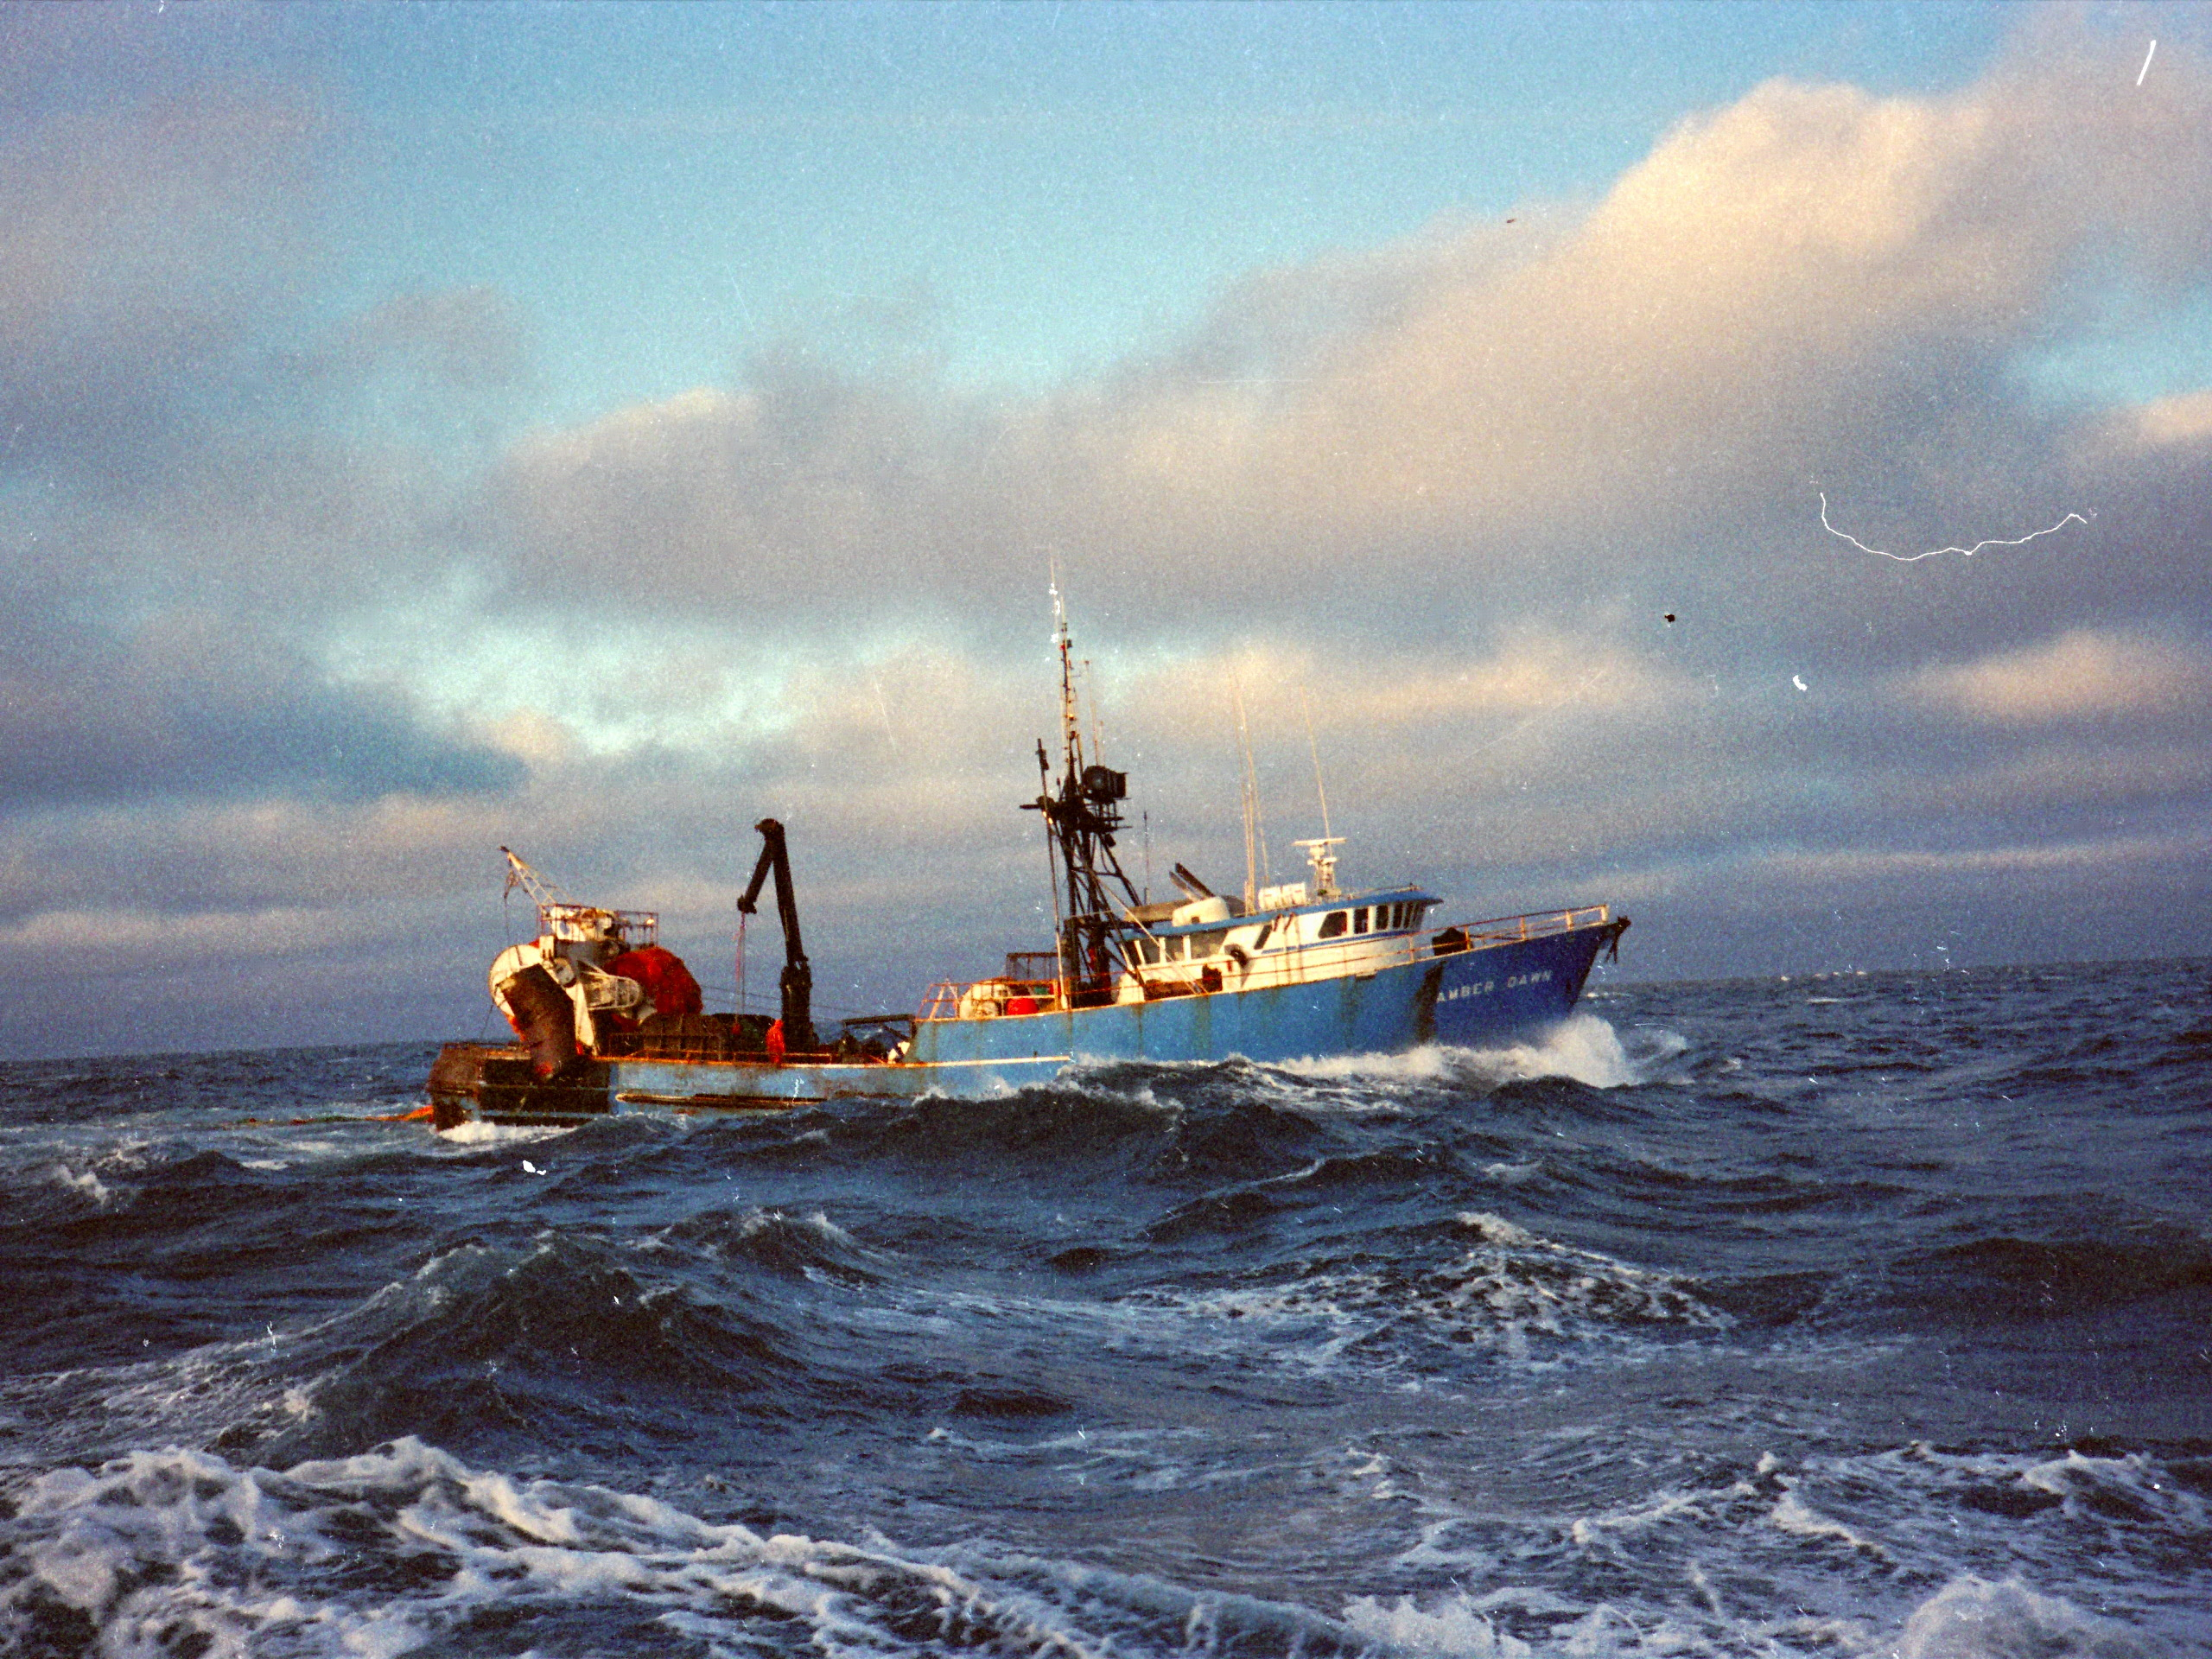
\includegraphics{BGbootAL},angle=0,scale=0.47,opacity=0.50,hshift=634}
\BgThispage
Het maken van een afstudeerproduct is een logische en verplichte laatste stap voor het afronden van mijn bacheloropleiding aan de Windesheim te Zwolle. Al voor de opdracht van start was gegaan was ik zeer geïnteresseerd om deze afstudeerstage uit te kunnen voeren bij een uitdagende en atypische opdrachtgever. Dit verlangen was vooral gegrond in het feit dat ik een affiniteit voor AO/BIV aan het ontwikkelen was en graag wilde toetsen of mijn kennis op dit vakgebied voldoende is. En waar beter deze kennis te toetsen dan bij een werkgever waar niet zomaar de geleerde typologieën gekopieerd en geplakt kunnen worden?
Mijn zoektocht begon naar een organisatie die in dit profiel past en graag met mij samen zou willen werken aan een nuttig eindproduct.

Eind juni kwam ik op de tennisbaan in gesprek met oud-collega Jurian, hier kwam Seafood Connection ter sprake als een interessante organisatie voor mij als afstudeerder. Al snel zat ik aan tafel met CFO Lucas Brouwer en voorgenoemde Jurian Molenaar waar Seafood Connection een steeds interessantere kandidaat leek te worden. Ik ben blij met de samenwerking die wij zijn aangegaan en ik hoop op een vruchtbare en productieve afstudeerperiode. Een bijzondere dank aan Rienk Bouma, Jon Bergsma, en Alidus Dannenberg voor de begeleiding vanuit school bij het formulerende proces van de opdracht. 

Ik wens de lezer veel plezier bij het lezen van dit afstudeerwerkplan en vanzelfsprekend ben ik bereid om vragen te beantwoorden en mee te nemen voor de opdracht.

\bigskip
\noindent
\textbf{Gerrit Post} \\
\textit{Student Accountancy, Hogeschool Windesheim}
